\chapter{Simulations d'ensemble} 

\section{Zones de diagnostic}
Au cours de cette étude, nous avons choisi de concentrer notre analyse sur quatre zones spécifiques, présentées en \autoref{fig:boxes}.

\begin{figure}[h]
\centering

\includegraphics[width=\textwidth]{Figures/bathy_zones}
\caption{Zones de diagnostics privilégiées}
\label{fig:boxes}
\end{figure}

Ces régions ont été sélectionnées afin d'assurer une couverture représentative de l’océan Indien sud-ouest, en englobant une diversité de régimes dynamiques.

La \autoref{fig:boxes} présente aussi la bathymétrie de notre zone d'étude. Nous constatons donc que cette région est parsemée de nombreuses iles, ainsi que d'un fort plateau continental, le plateau des Mascareignes.

La première zone est localisée à l’équateur, où l’influence de la force de Coriolis est négligeable. Cette région est traversée par des courants équatoriaux dont la direction s’inverse entre les deux saisons principales. Elle constitue ainsi un cadre idéal pour étudier les variations saisonnières ainsi que les processus dynamiques non géostrophiques.

La deuxième zone se situe au sud des Mascareignes, potentiellement influencée par la topographie et la présence d'îles (La Réunion, Maurice). Elle est dominée par un jet zonal intense, le courant subtropical sud-équatorial, et est soumise à des vents soutenus pendant une grande partie de l’année. Cette configuration en fait une région pertinente pour évaluer l’impact des perturbations du stress du vent sur la dynamique océanique.

La troisième zone comprend l’archipel des Comores, caractérisée par une bathymétrie complexe et fortement variable à petite échelle. L’étude de cette région vise à mieux comprendre l’effet du relief océanique sur la dynamique côtière..

Enfin, la quatrième zone est située au sud du canal du Mozambique, dans une région partiellement influencée par le courant des Aiguilles. Cette zone est stratégique pour le suivi de l’export de chaleur et de masse vers les latitudes tempérées.


\section{Évaluation des écarts simulation–observation}

Dans un premier temps, notre analyse porte sur la simulation déterministe, qui servira de référence pour évaluer la fidélité du modèle par rapport aux observations satellitaires. Les produits utilisés viennent du \textbf{CMEMS} et sont \textbf{OSTIA} pour la température de surface et \textbf{MOG} (Multi Observation Global) pour la salinité. Les données de température proviennent des satellites du projet \textbf{GHRSST}, tandis que celles de salinité sont issues des missions \textbf{SMOS} et \textbf{SMAP}.

L’évaluation est effectuée en calculant le biais moyen annuel pour l’année 2019, obtenu par la moyenne temporelle de l’écart entre les champs simulés et les observations. Ces biais sont présentés en \autoref{fig:bias}.

\begin{figure}[h]
\centering
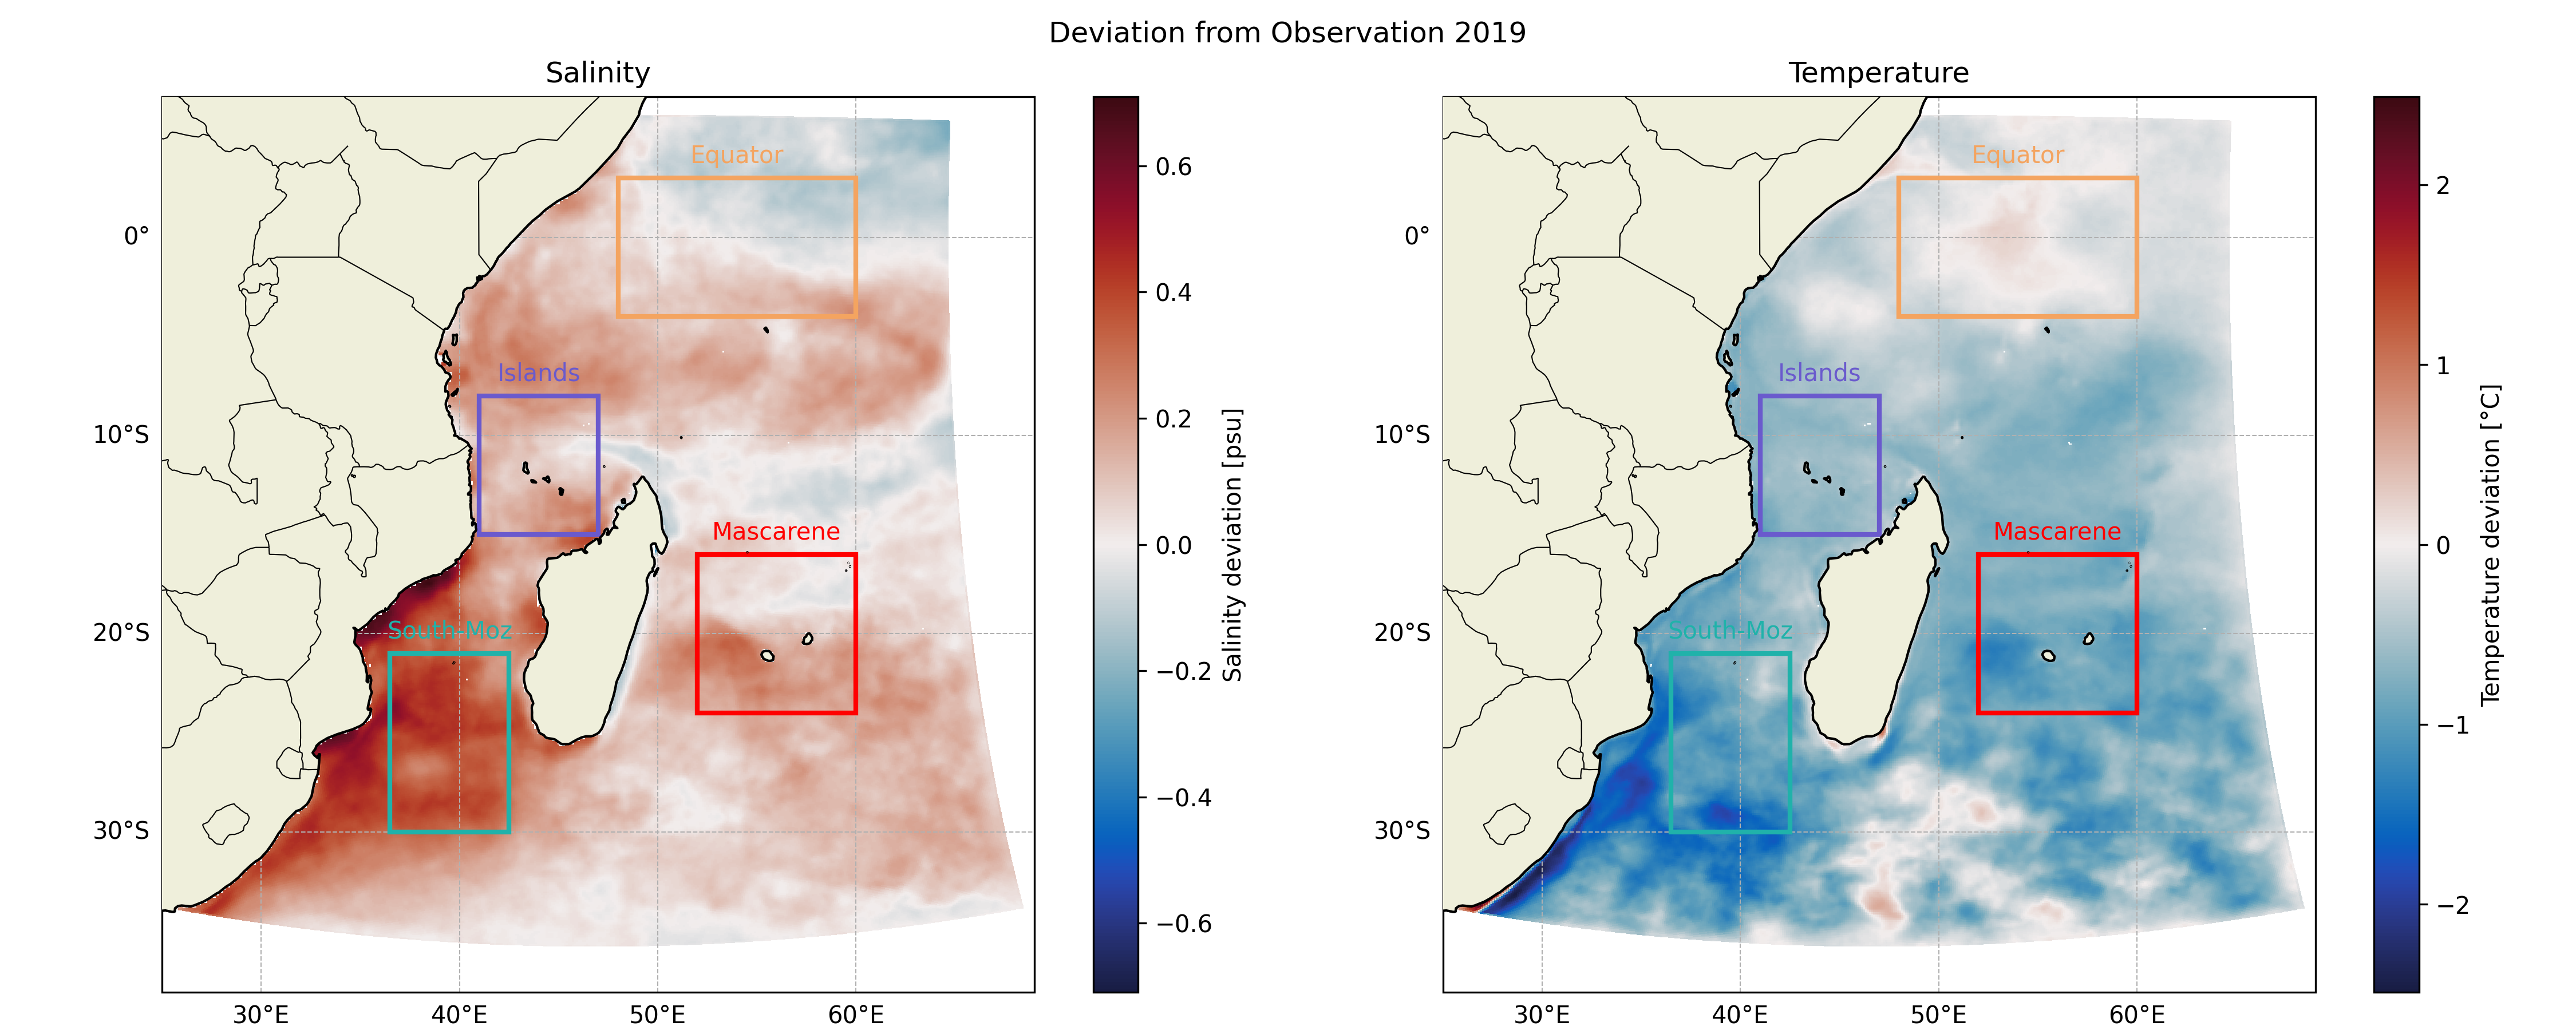
\includegraphics[width=\textwidth]{Figures/deviation_obs_2019_deter}
\caption{Biais moyen de la simulation par rapport aux observations}
\label{fig:bias}
\end{figure}

L’analyse de cette figure révèle deux résultats notables. D’une part, la température présente un biais fortement négatif sur l’ensemble du domaine. Ce comportement peut s’expliquer par le biais négatif bien documenté du forçage atmosphérique \textbf{ERA5} sur la température de l’air. D’autre part, un biais positif marqué sur la salinité apparaît dans le canal du Mozambique, ce qui résulte principalement de l’absence de prise en compte des apports fluviaux dans la configuration actuelle du modèle.

Ces écarts montrent la nécessité d’une correction des biais structurels avant d’entreprendre des études à visée réaliste. Dans la suite de ce travail, nous allons donc nous concentrer sur une étude de sensibilité du modèle face à différentes sources de perturbation.

\section{Dispersion des traceurs}

Nous allons maintenant analyser les ensembles de simulation. Une première approche consiste à observer les séries temporelles des traceurs, ce qui permet d’évaluer la cohérence des dynamiques reproduites par chaque ensemble. La \autoref{fig:salt} présente l’évolution de la salinité de surface pour la zone \textit{Islands} en fonction du temps. Ici il s'agit de la valeur de surface moyennée dans l'entièreté de la zone à chaque instant.

\begin{figure}[h]
\centering
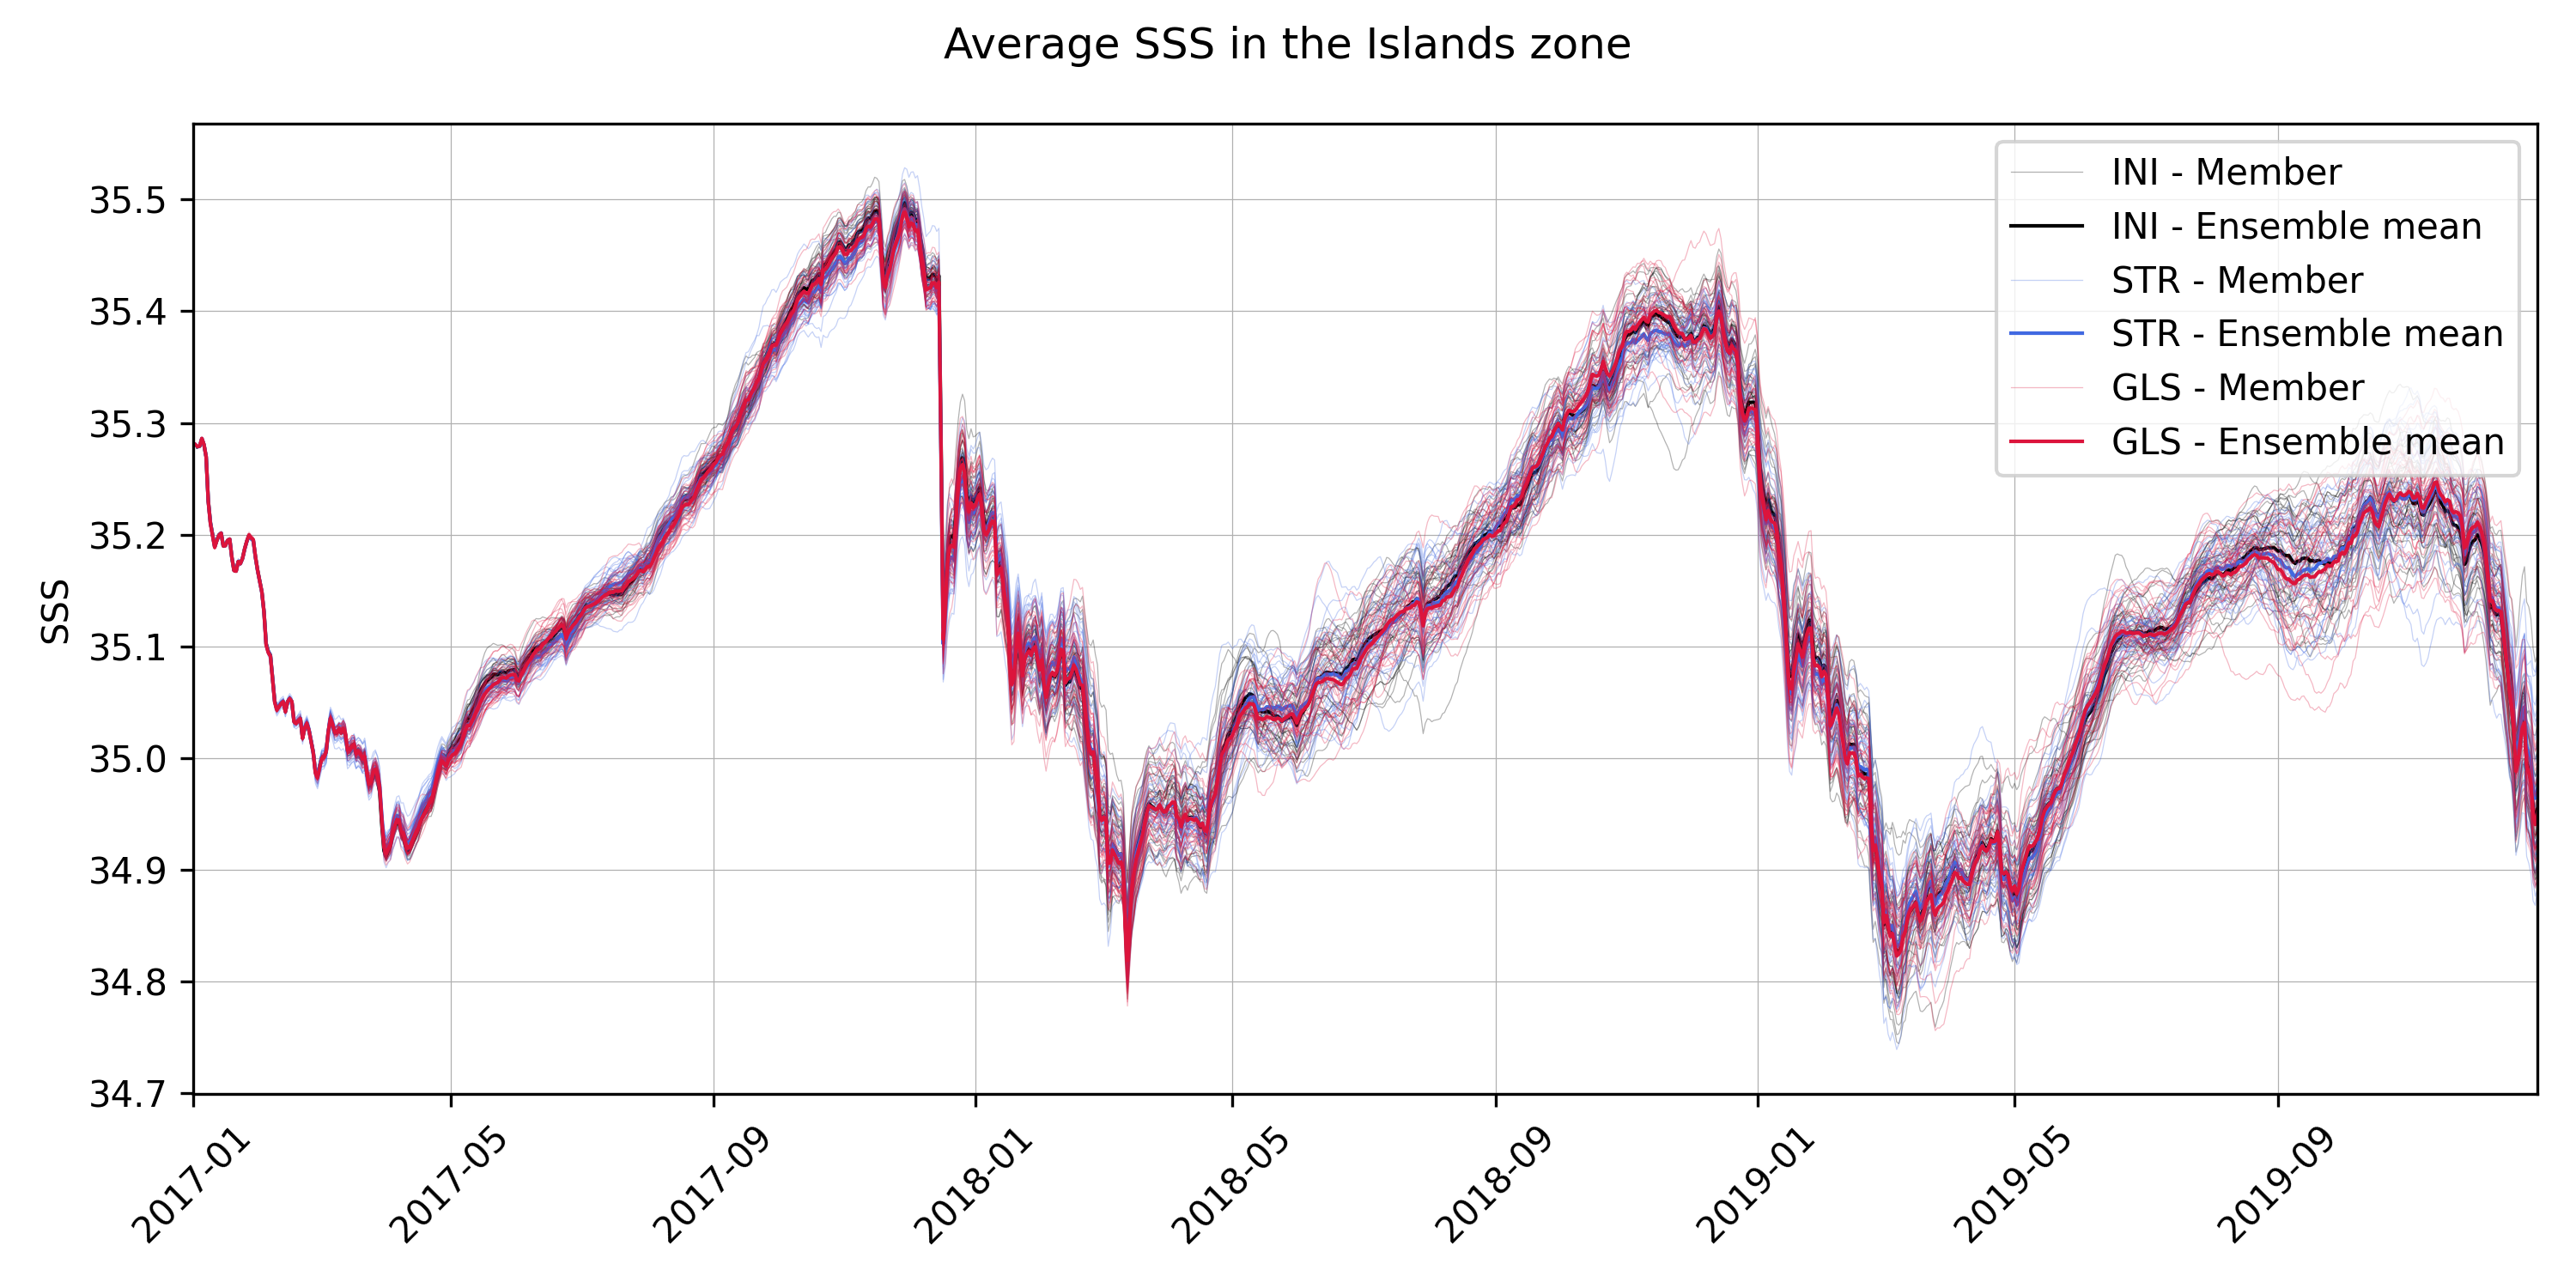
\includegraphics[width=\textwidth]{Figures/all_ens_Islands_salt}
\caption{Série temporelle de la salinité de surface pour la zone \textit{Islands}}
\label{fig:salt}
\end{figure}

L’analyse de cette figure montre que tous les ensembles suivent une dynamique moyenne très similaire. Cela suggère que, malgré les perturbations spécifiques introduites dans chaque configuration, la structure globale de salinité reste robuste. On observe néanmoins quelques divergences ponctuelles, notamment lors de transitions de saison. Par ailleurs, les cycles saisonniers sont bien marqués et reproduits de façon cohérente dans chaque ensemble, ce qui valide le bon comportement du système à grande échelle.

Nous voulons ensuite étudier la dispersion\footnote{Ici le mot dispersion correspond à l'écart-type d'ensemble de la variable} de la salinité dans cette même zone, en \autoref{fig:salt disperion}. Cette figure présente la dispersion des ensembles moyennée sur la boite avec plus ou moins l'écart-type d'ensemble. 

\begin{figure}[h]
\centering
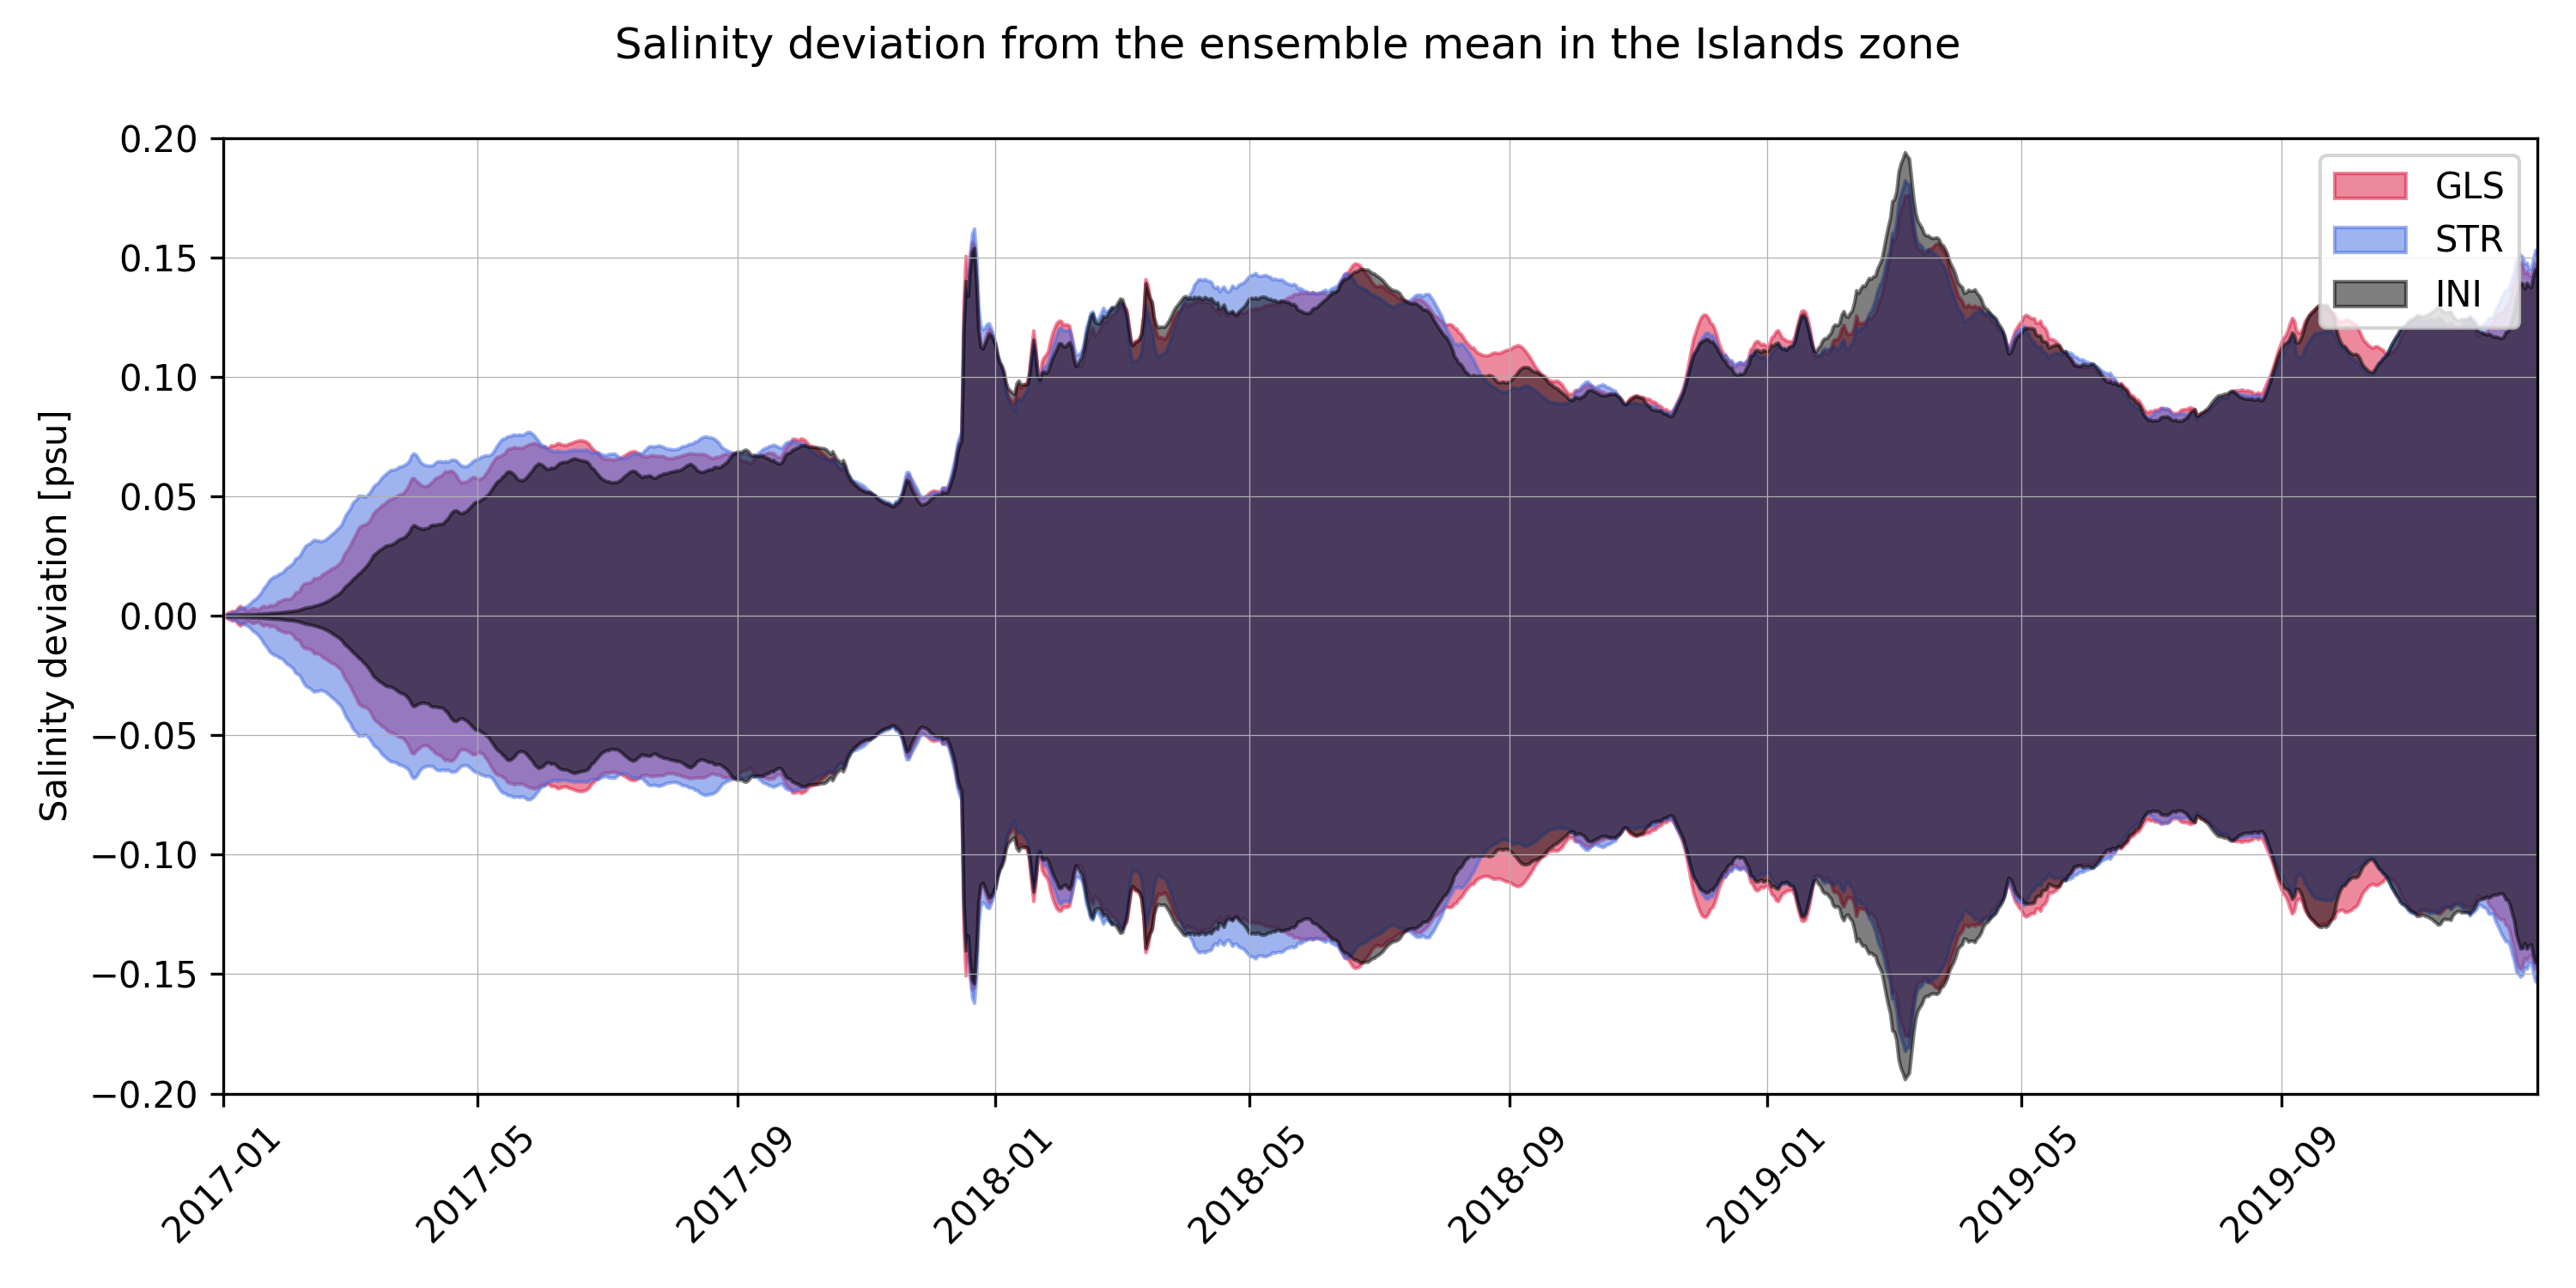
\includegraphics[width=\textwidth]{Figures/all_ens_Islands_salt_deviation}
\caption{Série temporelle de la dispersion de salinité de surface pour la zone \textit{Islands}}
\label{fig:salt dispersion}
\end{figure}

Contrairement à l'analyse précédente portant sur la moyenne, cette fois des différences significatives apparaissent entre les ensembles. La plus notable est la phase transitoire observée sur les 6 premiers mois de simulation, nettement plus courte dans l'ensemble \textbf{STR} que dans les deux autres.

Un point important à souligner à partir de cette figure est la faible dispersion relative entre les ensembles une fois la phase transitoire terminée. Cela met en évidence le rôle dominant de la variabilité intrinsèque du modèle, qui crée une enveloppe de référence dans laquelle les autres ensembles ne s’écartent que faiblement.

En revanche, on note l'absence de cycle saisonnier marqué pour la salinité dans cette zone. Pour approfondir cette question, nous allons examiner la température dans une autre région, la zone \textit{Equator}, présentée en \autoref{fig:temp disperion}, afin d'identifier d'éventuelles variations régionales dans le comportement des traceurs. Ici encore, nous présentons la dispersion des ensembles de la même manière que précédemment.

Cette fois, les durées des phases transitoires des ensembles \textbf{STR} et \textbf{GLS} sont similaires. La différence porte principalement sur l'amplitude de la dispersion : le modèle de mélange vertical semble générer une dispersion plus importante que celle induite par la perturbation du coefficient de stress du vent dans cette zone.

\begin{figure}[h]
\centering
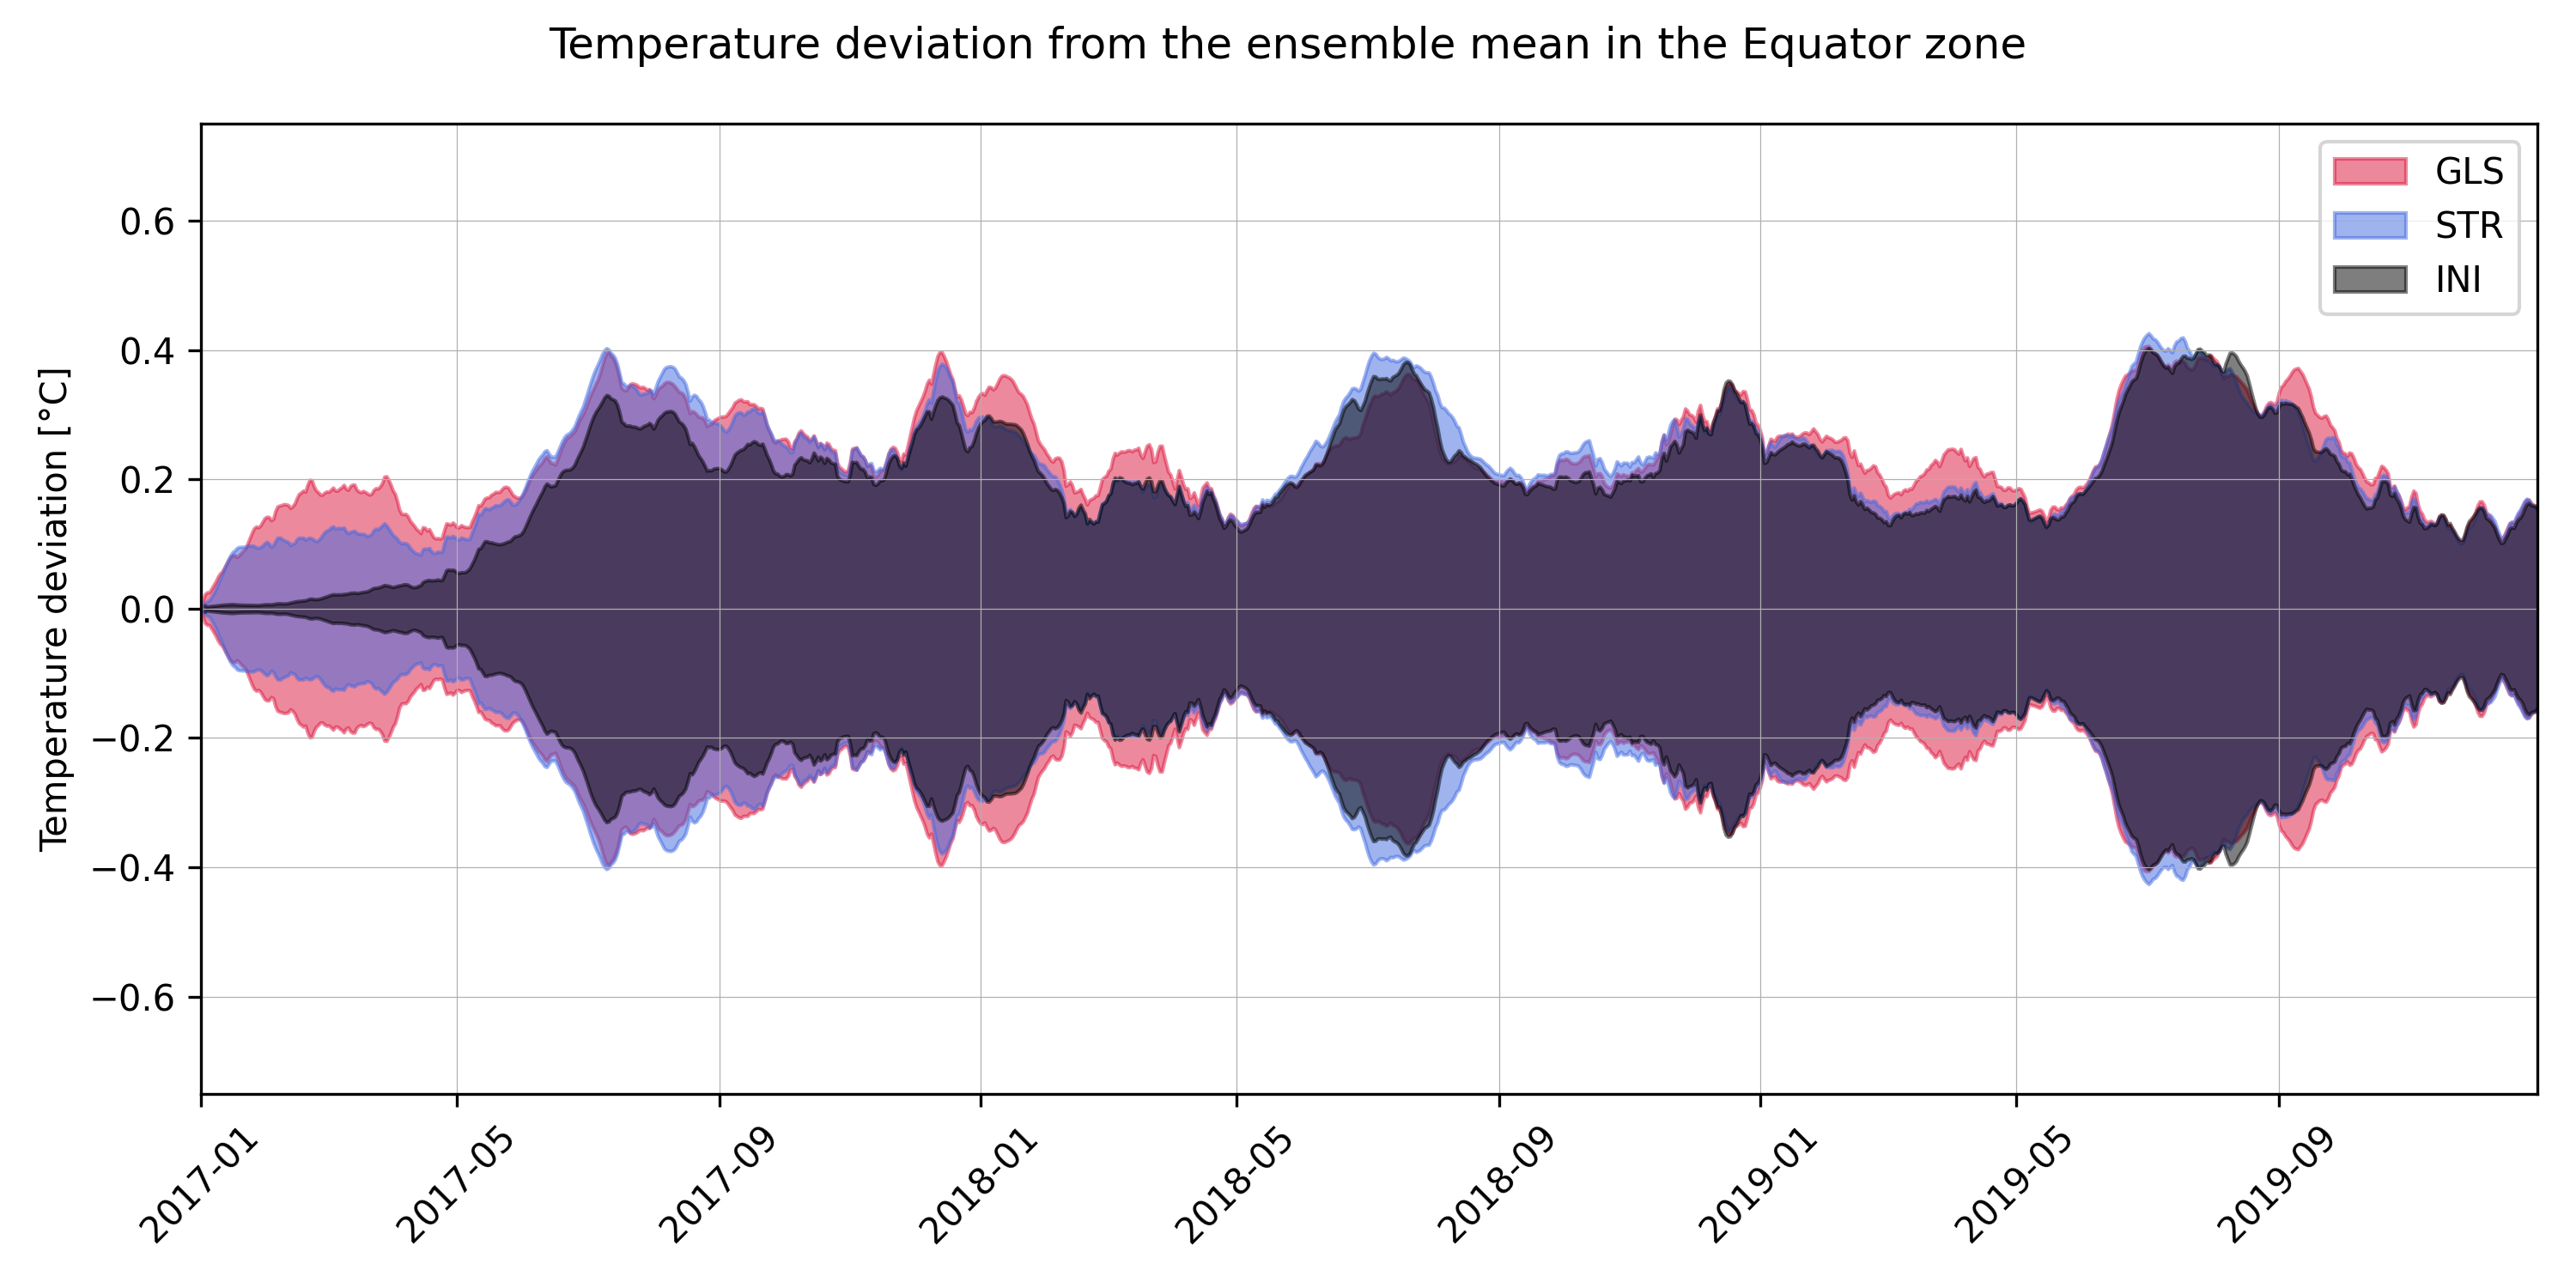
\includegraphics[width=\textwidth]{Figures/all_ens_Equator_temp_deviation}
\caption{Série temporelle de la dispersion de température de surface pour la zone \textit{Equator}}
\label{fig:temp disperion}
\end{figure}

Dans cette région équatoriale, nous observons également des cycles saisonniers marqués de la dispersion de la température. Des déphasages apparaissent entre certains ensembles. L'ensemble \textbf{STR} génère une dispersion plus prononcée durant les mois de juin à septembre, tandis que l'ensemble \textbf{GLS} présente une dispersion maximale sur la période de janvier à avril.

Ces comportements sont cohérents avec la configuration des courants présentée en \autoref{fig:currents}. Durant les premiers mois de l'année, le courant de Somalie et le courant côtier d'Afrique de l'Est convergent, formant le courant subéquatorial (\autoref{fig:JFM current}). Cette interaction génère de nombreux tourbillons de méso-échelle, qui influencent fortement le mélange vertical. À l’inverse, durant l’été austral (\autoref{fig:JJA current}), les vents sont renforcés en raison de l’alignement des grands courants, ce qui augmente l’effet des perturbations sur le coefficient de stress du vent.

Ces divergences illustrent clairement l’impact de différentes sources d’incertitude dans la résolution numérique de la circulation océanique. Lorsque la dynamique est dominée par le vent, une perturbation du coefficient de stress induit une variabilité accrue. À l’inverse, en présence de tourbillons de méso-échelle, ce sont les termes de production et de destruction de la turbulence dans la paramétrisation de la \textbf{TKE} (Turbulent Kinetic Energy) qui deviennent prépondérants dans l’amplification de la dispersion.

\begin{figure}[h]
     \centering
     \begin{subfigure}[b]{0.49\textwidth}
         \centering
         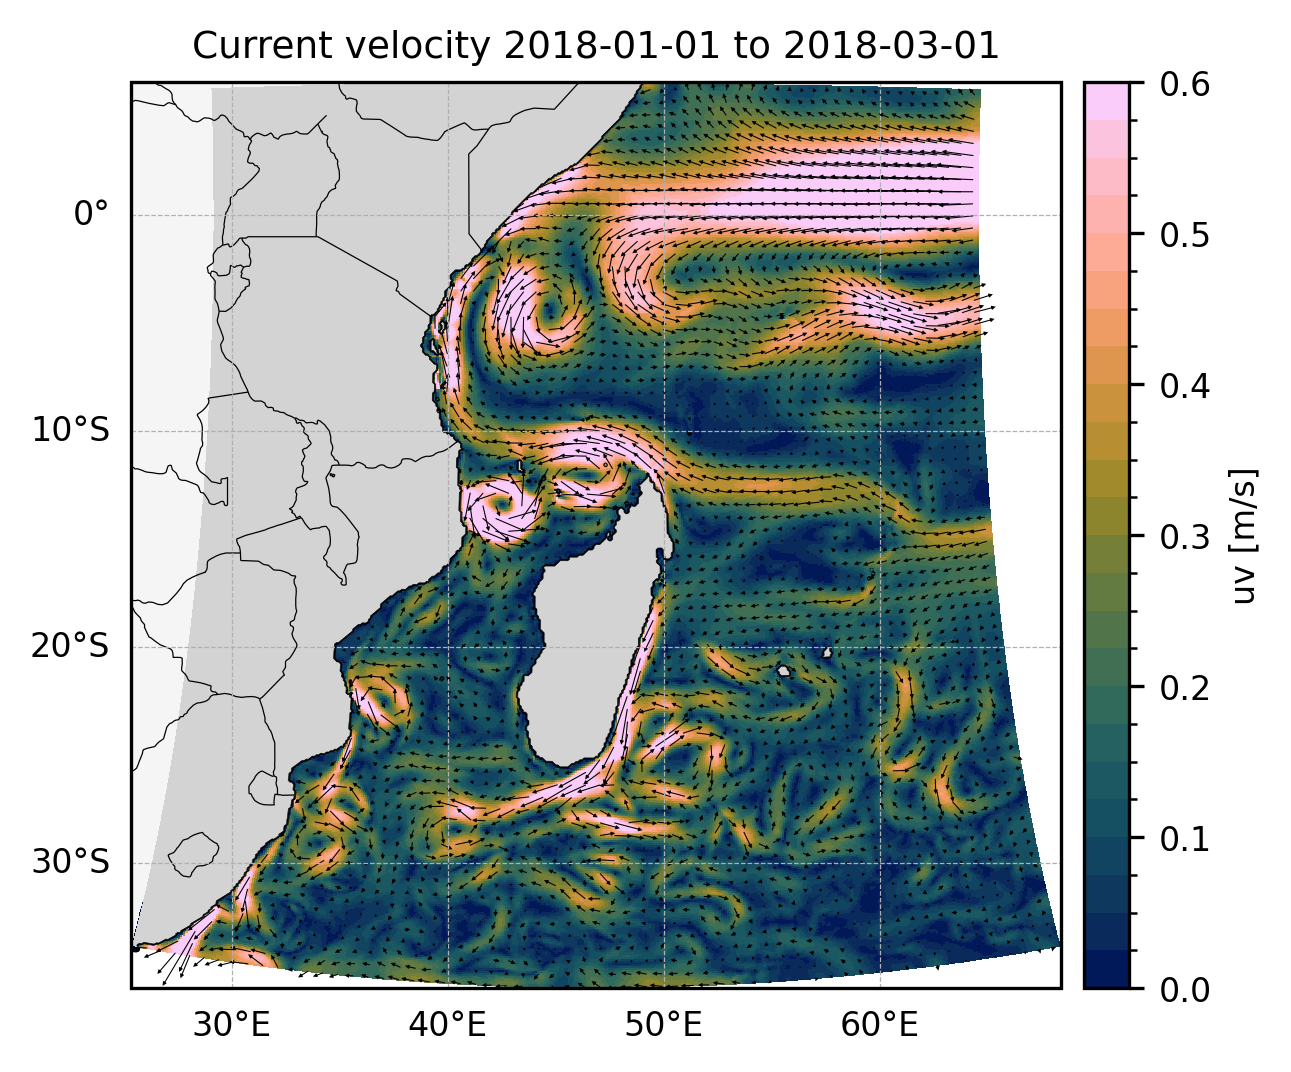
\includegraphics[width=0.8\textwidth]{Figures/uv_2018-01-01_2018-03-01}
         \caption{Du 1\textsuperscript{er} janvier 2018 au 1\textsuperscript{er} mars 2018}
         \label{fig:JFM current}
     \end{subfigure}
     \hfill
     \begin{subfigure}[b]{0.49\textwidth}
         \centering
         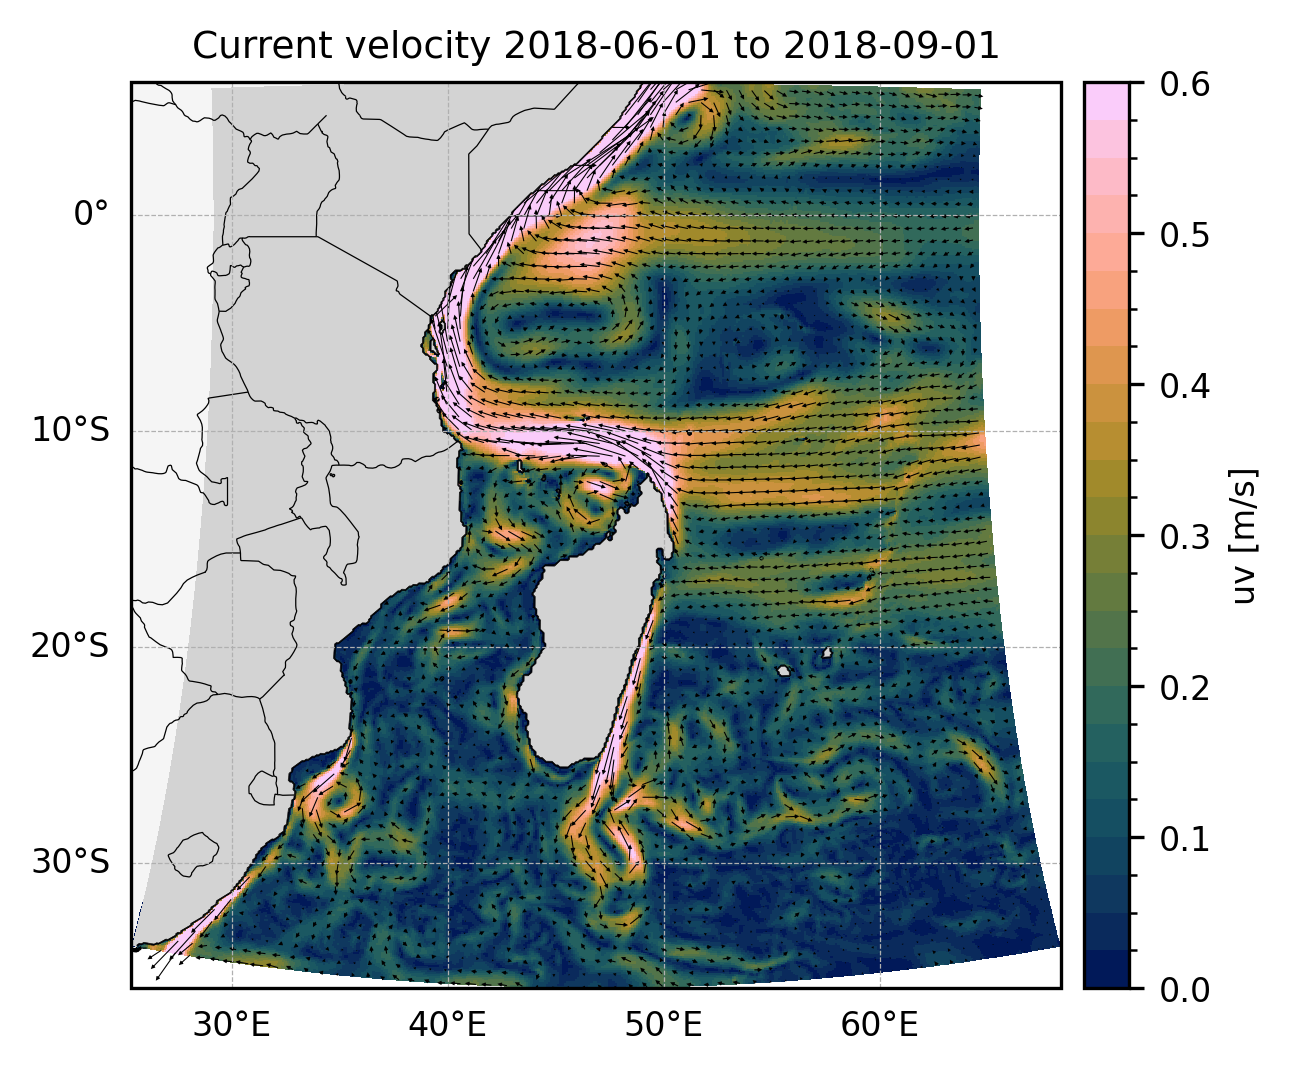
\includegraphics[width=0.8\textwidth]{Figures/uv_2018-06-01_2018-09-01}
         \caption{Du 1\textsuperscript{er} juin 2018 au 1\textsuperscript{er} septembre 2018}
         \label{fig:JJA current}
     \end{subfigure}
     \caption{Courant moyen de surface sur deux périodes représentatives de l'année 2018}
     \label{fig:currents}
\end{figure}

Après avoir étudié les traceurs tels que la salinité et la température, nous nous intéressons désormais à une variable présentant une forte variabilité spatiale et temporelle : la profondeur de la couche de mélange.

\section{Dispersion de la couche de mélange}

Une variable encore peu diagnostiquée dans des simulations ensemblistes, mais présentant une forte variabilité, est la profondeur de la couche de mélange, appelée \textbf{Mixing Layer Depth} ou \textbf{MLD} en anglais. Nous allons donc détailler la méthode de calcul de cette variable, puis analyser les différents profils et l’évolution temporelle de cette profondeur.

\begin{wrapfigure}{r}{0.5\textwidth}	
\centering
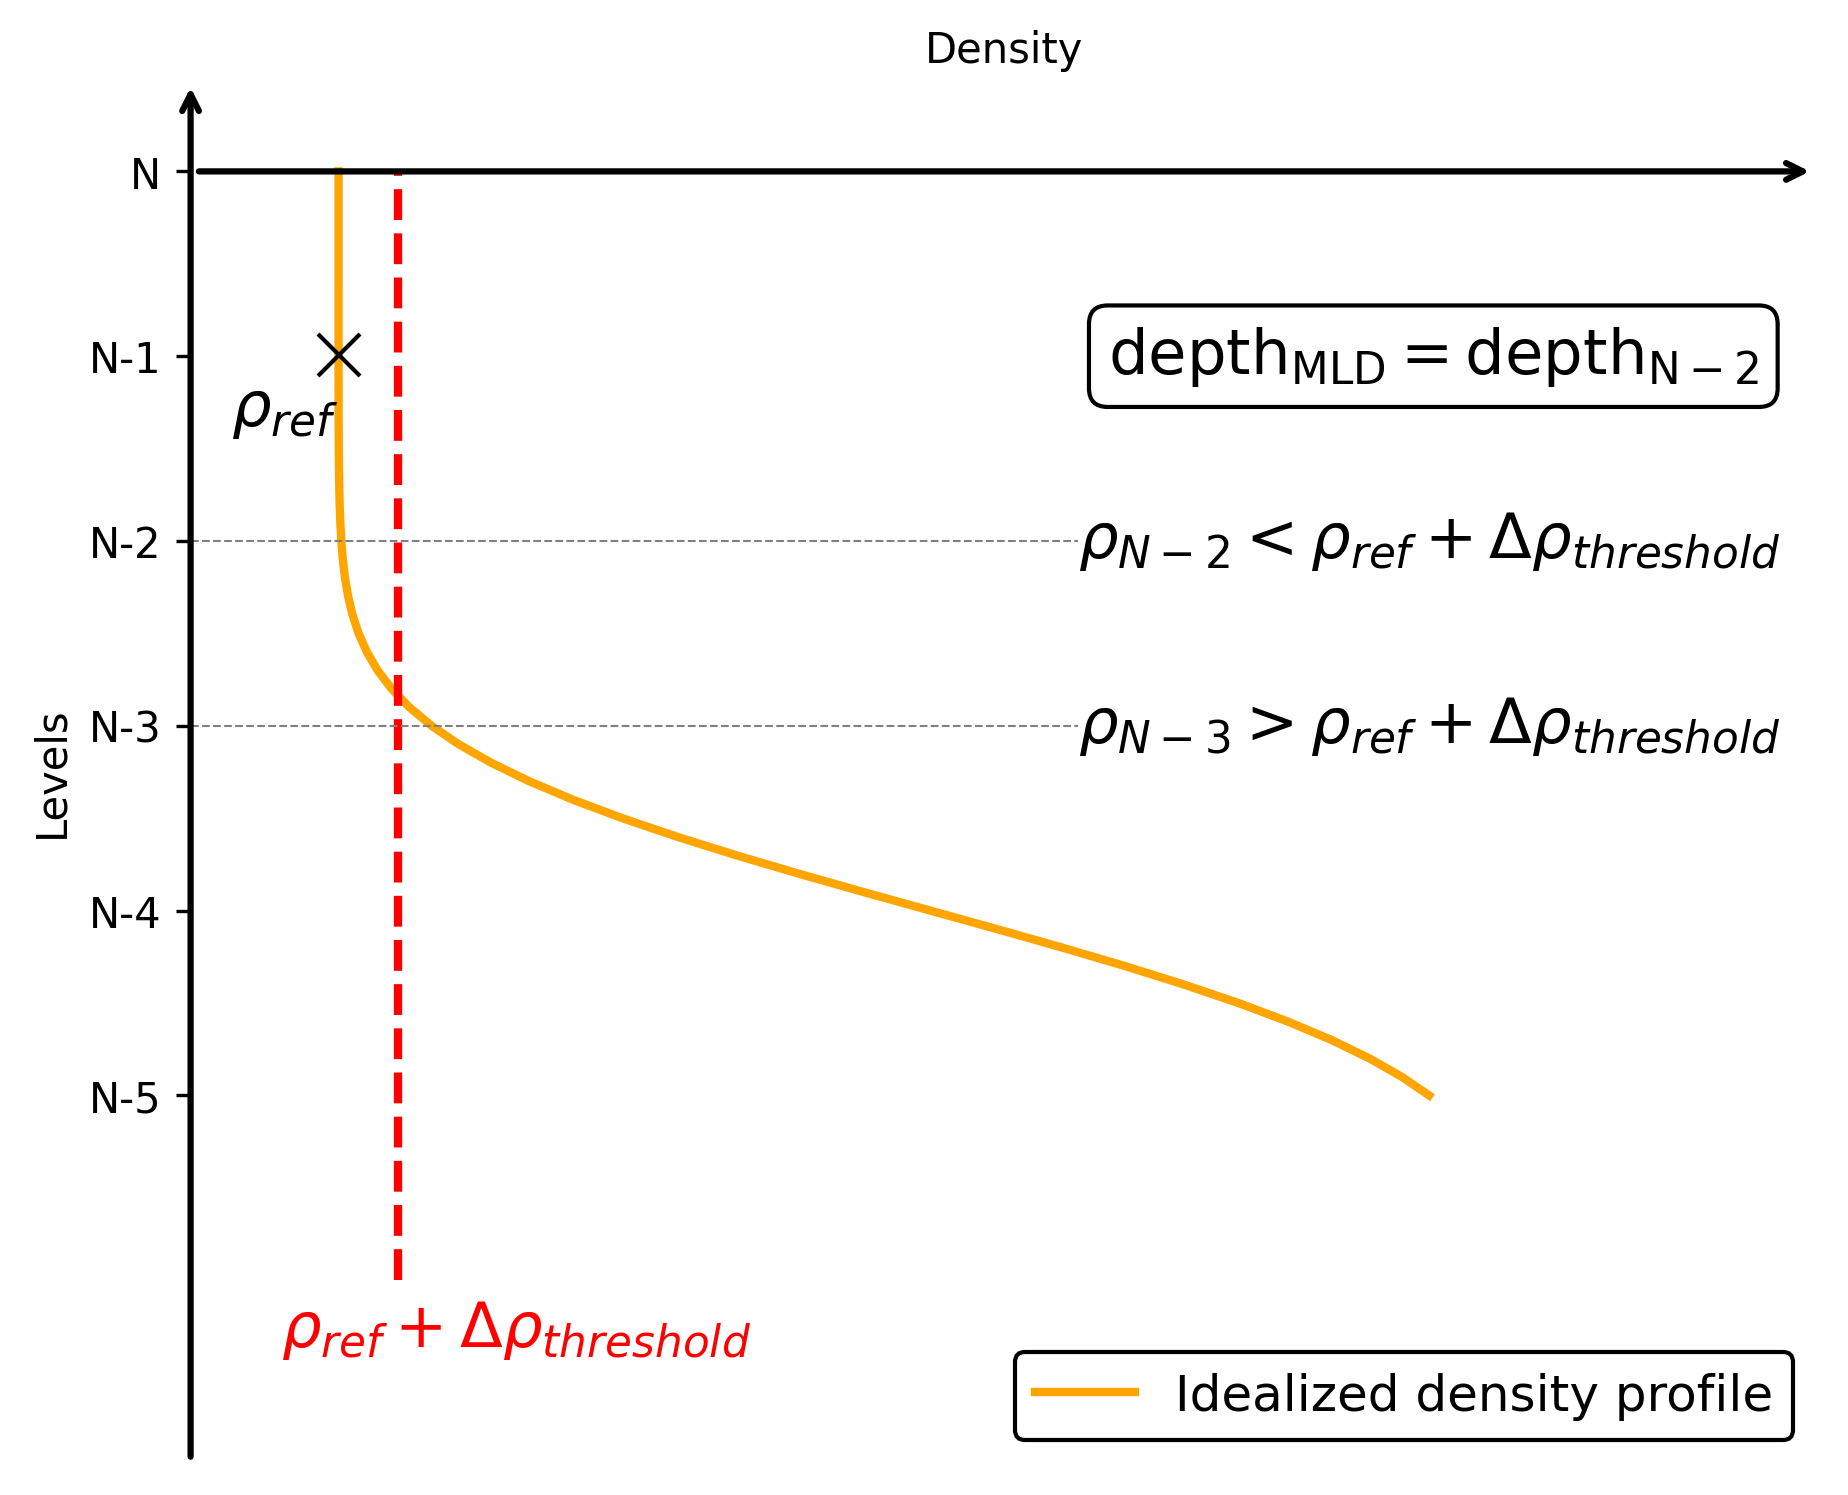
\includegraphics[width=0.5\textwidth]{Figures/MLD_def}
\caption{Calcul de la profondeur de mélange}
\label{fig:mld def}
\end{wrapfigure}

\subsection{Définition}

La \textbf{MLD} est une variable dépendant directement du profil vertical de densité, comme illustré en \autoref{fig:mld def}, ce qui lui confère une variabilité prononcée. Sa définition repose sur une méthode de seuil : la profondeur considérée correspond au premier niveau $z$ pour lequel la densité $\rho(z)$ dépasse une densité de référence $\rho_{\text{ref}}$ (typiquement mesurée à \SI{10}{\meter}) augmentée d’un seuil $\Delta \rho_{\text{threshold}} = \SI{0.03}{\kilo\gram\per\meter\cubed}$, tel que proposé par \cite{de_boyer_montegut_mixed_2004}.

Bien que la profondeur de la couche de mélange ne soit pas une sortie directe du modèle, elle peut être estimée de manière fiable à partir des profils simulés de densité. Pour cela, nous utilisons une interpolation linéaire entre les niveaux verticaux, ce qui permet d’éviter une quantification trop grossière liée à la discrétisation verticale fixe du modèle. 

Il est toutefois important de noter que cette interpolation linéaire reste une approximation : une méthode plus précise consisterait à ajuster une fonction plus réaliste (ex. spline, ajustement polynomial local) à l'évolution verticale de la densité afin de mieux capturer la transition entre la couche de surface homogène et la thermocline. Cette couche de mélange existe du fait de l'interaction avec l'air de l'atmosphère qui mélange les couches proches de la surface, mais aussi par les courants générés par le vent.

\subsection{Résultats}

\begin{wrapfigure}{r}{0.4\textwidth}	
\centering
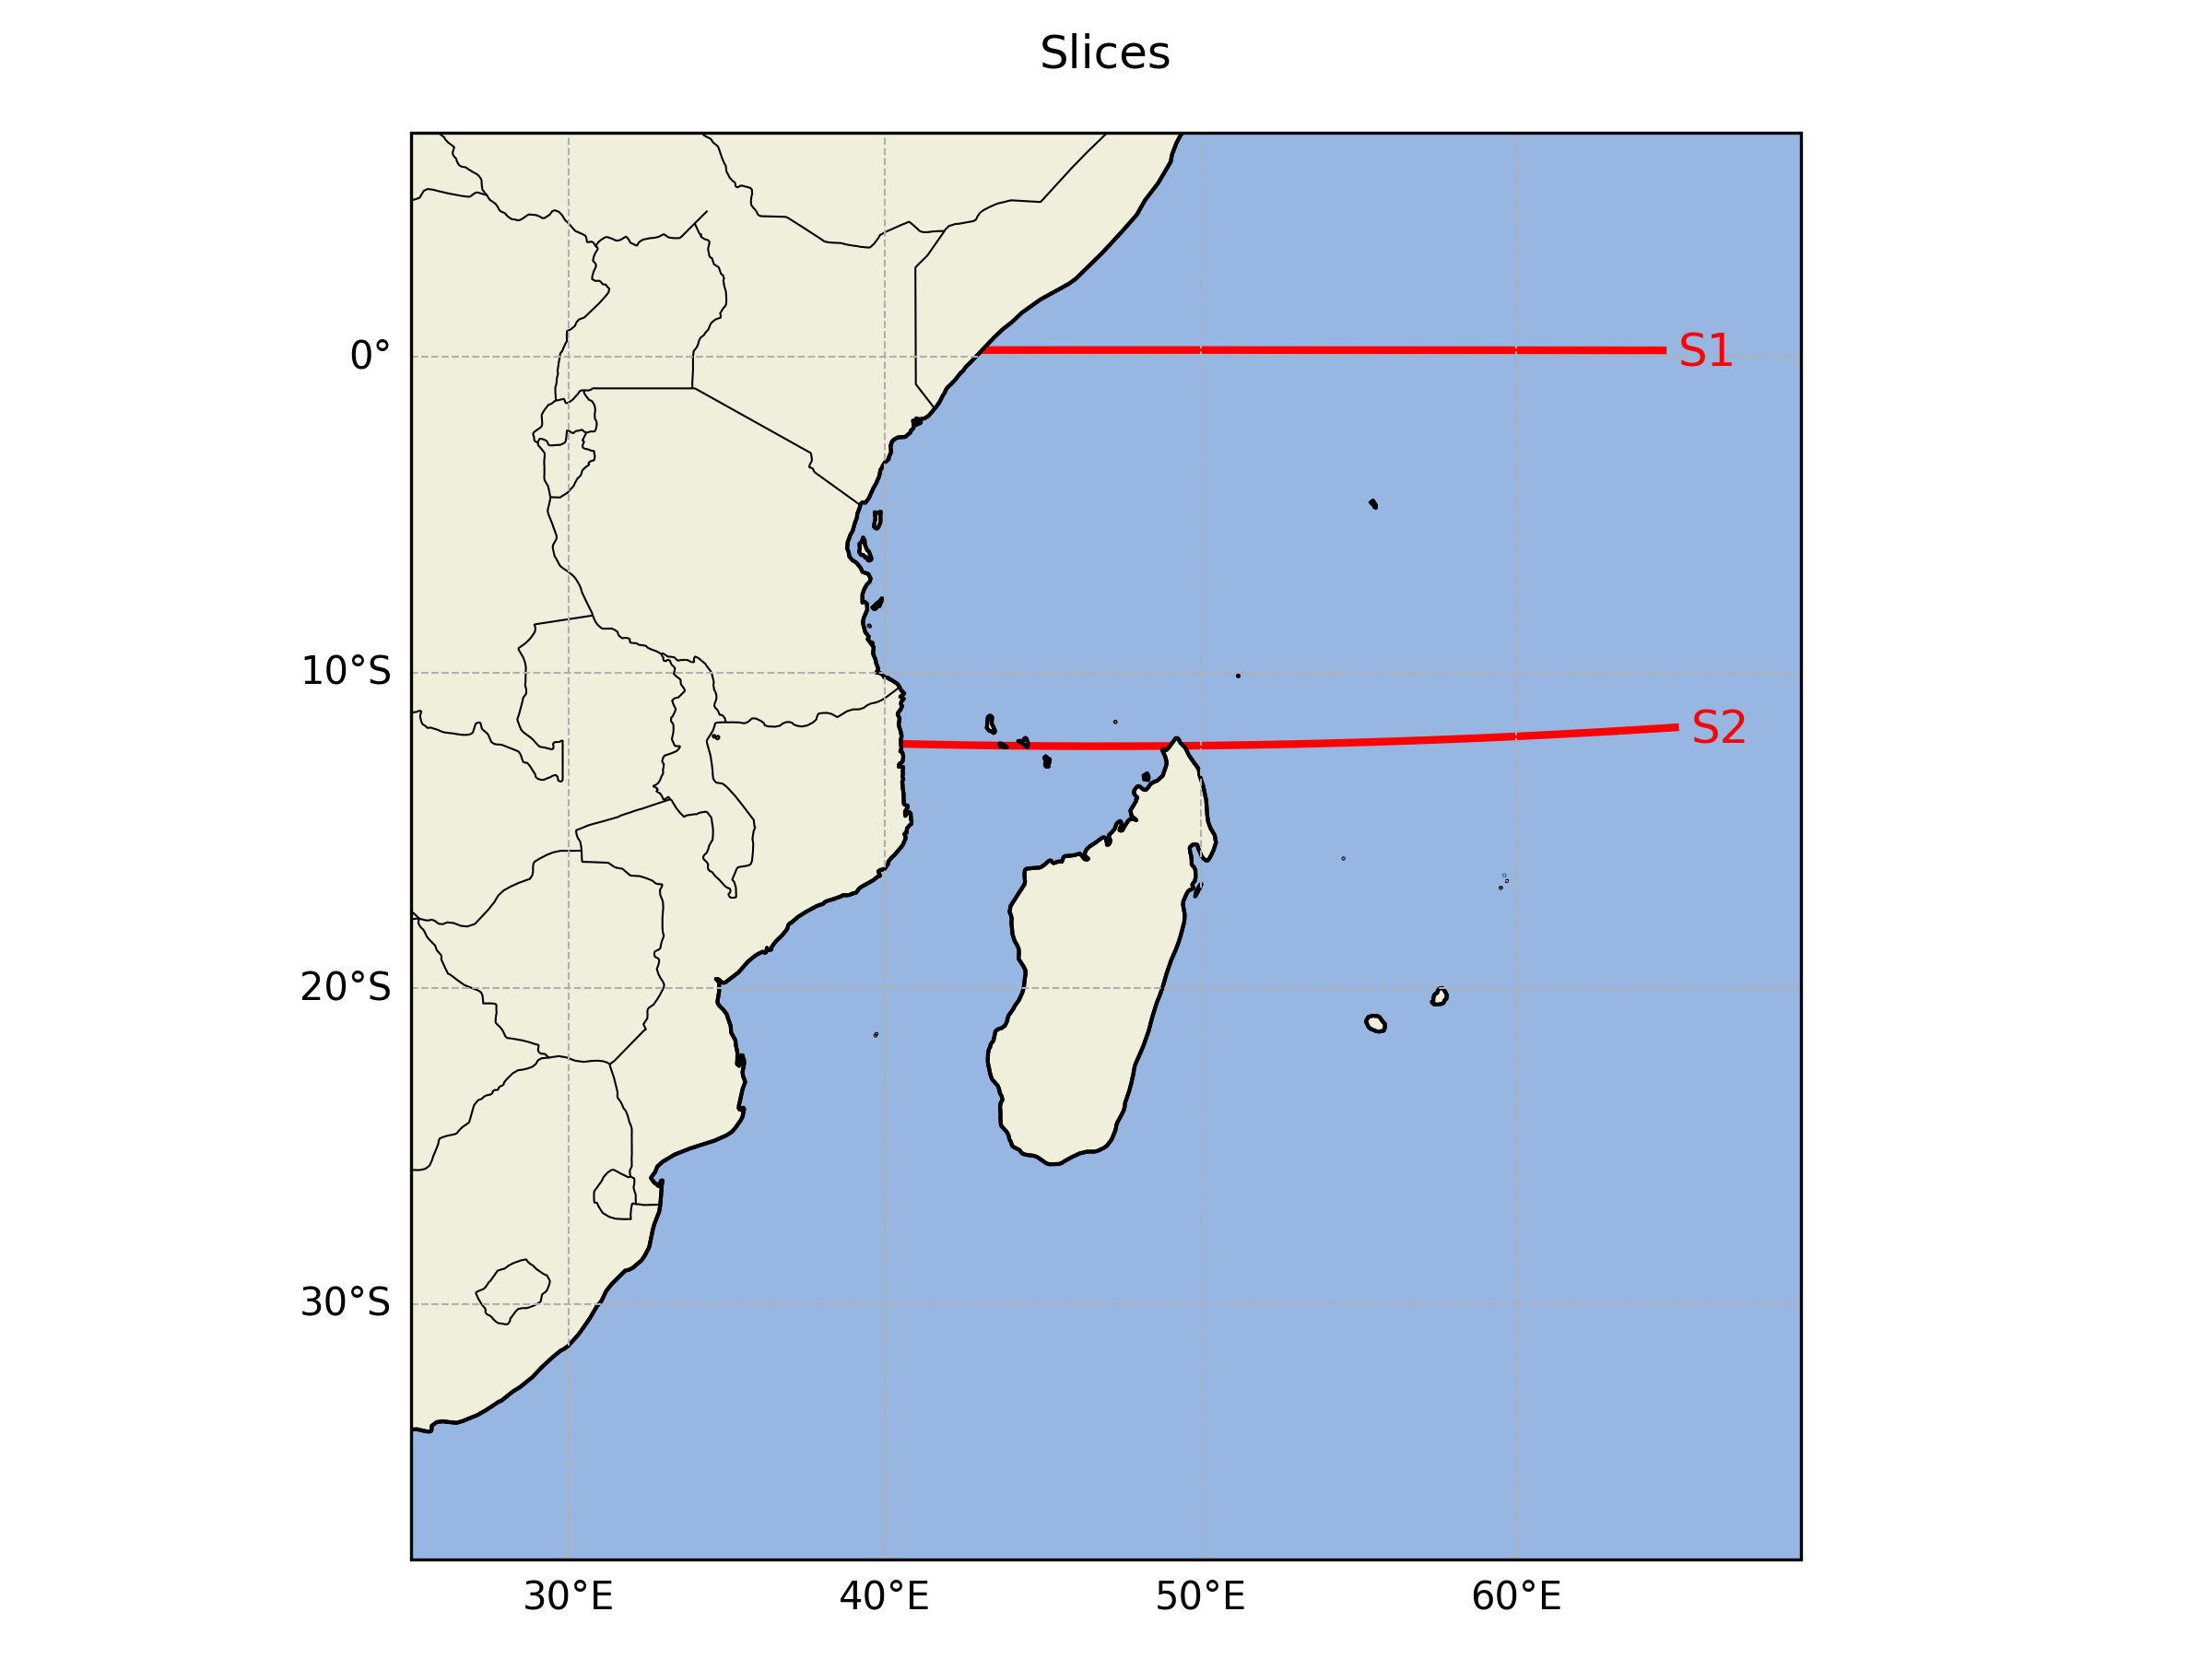
\includegraphics[width=0.4\textwidth]{Figures/slice}
\caption{Position des coupes zonales}
\label{fig:slice}
\end{wrapfigure}

Dans un premier temps, nous analysons des coupes verticales de la \textbf{MLD}, représentées en \autoref{fig:slice}. Ces coupes permettent d’identifier les zones présentant une variabilité marquée, ainsi que d’obtenir une vision verticale et spatiale de l’évolution de cette variable. Deux transects ont été choisis : l’un à l’équateur, afin d’examiner l’effet de l’absence de composante géostrophique ; l’autre au nord de Madagascar, dans une région de bathymétrie complexe, pour évaluer son impact sur la dispersion.

Sur la \autoref{fig:mld slice}, nous présentons la profondeur moyenne de la couche de mélange pour chaque ensemble en trait gras, ainsi que la valeur de chaque membre en trait fin. La coupe équatoriale montre une dispersion relativement homogène sur l’ensemble du domaine, à l’exception de la frontière ouest, où les membres convergent fortement. Ce comportement s’explique par l’influence du forçage aux frontières, qui impose une contrainte forte sur le profil de densité. On observe également une augmentation de la dispersion à proximité du continent africain, en lien avec la présence du courant de Somalie, lequel intensifie le mélange vertical.

\begin{figure}[h]
\centering
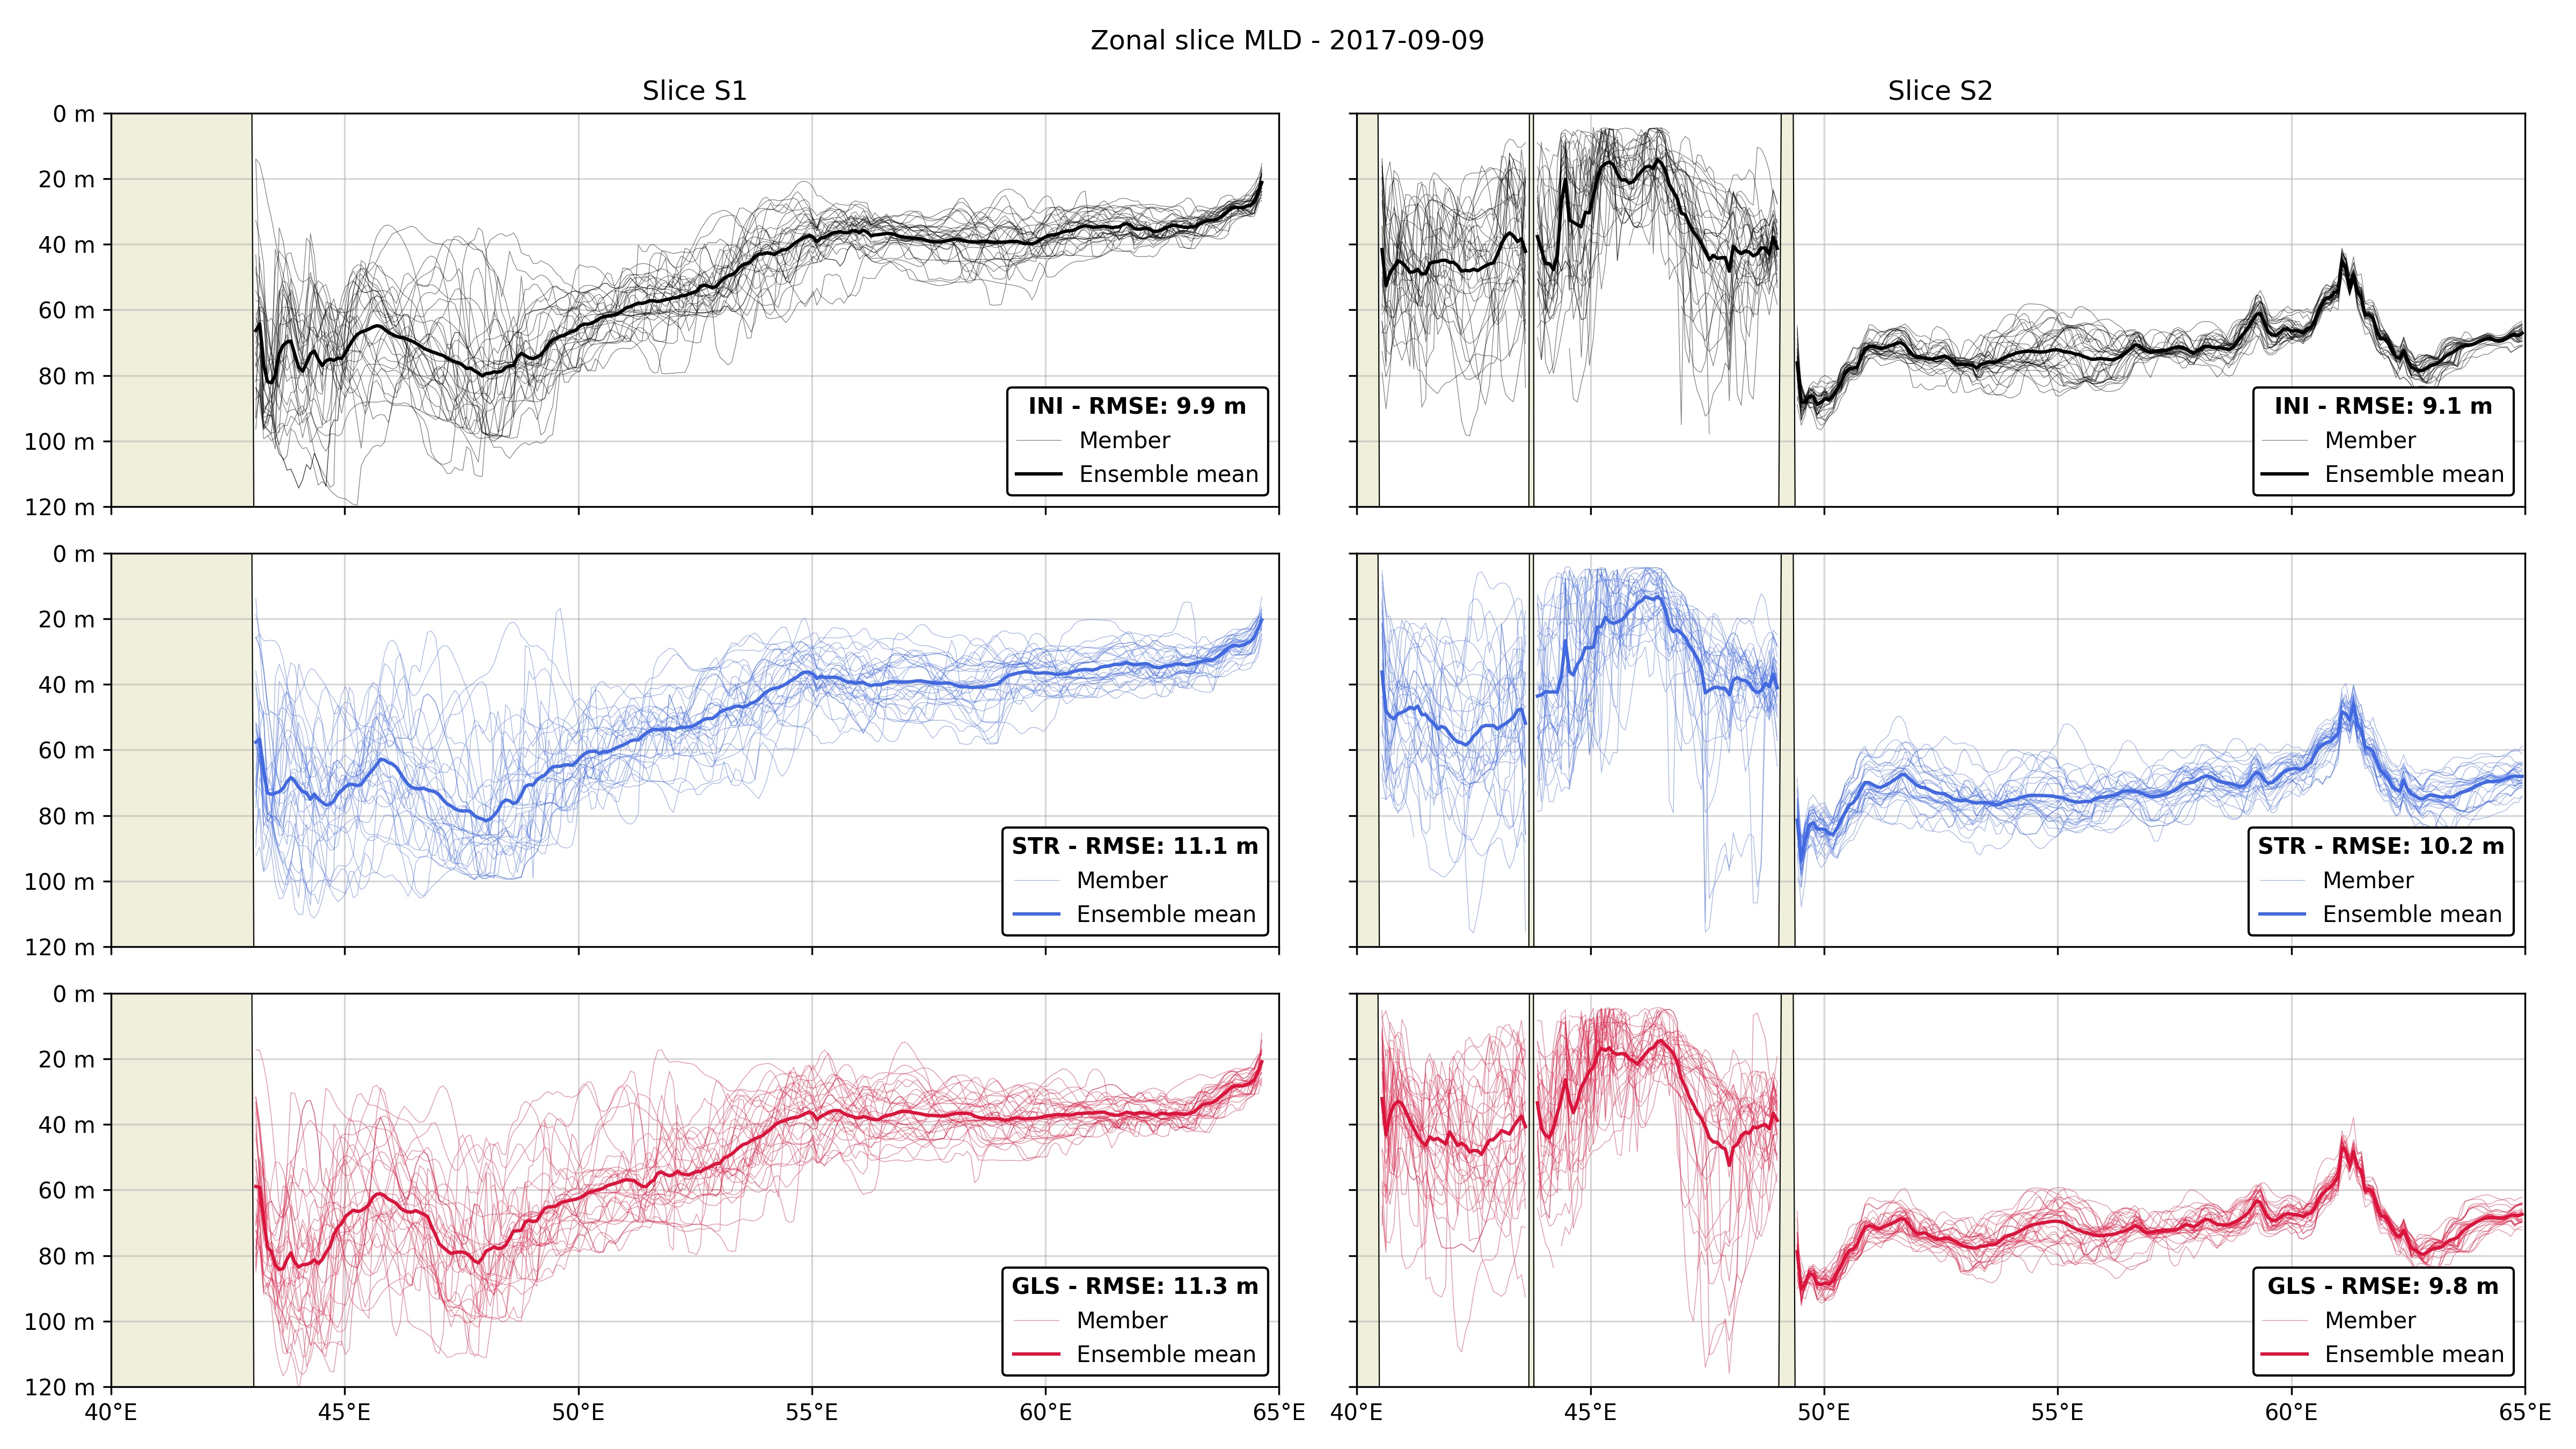
\includegraphics[width=\textwidth]{Figures/slices_mld_comp_2017-09-09}
\caption{Coupes zonales de la \textbf{MLD} pour chaque ensemble}
\label{fig:mld slice}
\end{figure}

La seconde coupe révèle deux régimes bien distincts : 
\begin{itemize}
    \item entre le continent africain et Madagascar, la dispersion atteint des valeurs élevées, de l’ordre de \SI{15}{\meter} pour tous les ensembles,
    \item à l’est de Madagascar, cette dispersion chute aux alentours de \SI{4}{\meter}.
\end{itemize}

Cette différence reflète l’effet combiné de la bathymétrie complexe et de l’un des jets qui contourne Madagascar sur le développement de la variabilité verticale. Il est également important de noter que l’ensemble \textbf{INI} présente systématiquement une dispersion plus faible que les ensembles \textbf{STR} et \textbf{GLS}, et ce aussi bien dans les deux coupes (S1 et S2) que dans les deux régimes identifiés de la seconde coupe.

\section{Conclusion}

Cette étude a permis d’identifier les impacts différenciés des perturbations introduites dans nos ensembles de simulation. Ces perturbations ne se traduisent pas simplement par une augmentation uniforme de la dispersion, mais peuvent générer des effets localisés, aussi bien spatialement que temporellement, sur la variabilité d’une variable donnée.

Nous avons montré que les incertitudes introduites par les perturbations s’ajoutent à la variabilité intrinsèque du modèle, sans toutefois la dominer. En effet, cette variabilité intrinsèque structure l’enveloppe moyenne de la dispersion et constitue le socle sur lequel les autres sources d’incertitude viennent moduler la réponse du système. Cela est du à la nature chaotique du système qui est bien représenté par la haute résolution utilisée (1/12\degree) ce qui génère une méso-échelle intense.


